\section{有向线段}

有向线段或箭头在欧几里德几何中是基石一般的存在。从数学角度来讲,箭头就是一对有序的点$(A,B)$。A点是箭的尾端,B点是箭的首端。通常将这样的箭头在印刷上表示为$\rr{AB}$,在图形上表示为从A到B的线段,箭头指向 B。(为避免拥挤,箭头可能会移向线段的中心)。 在$E_3$中,为箭头指定长度或将其乘以一个实数(保持尾部固定)是精确定义的操作。

如果一个箭头可以通过平移使其与另一个箭头完全重合,那么我们就可以说两个箭头是相等的\footnote{这是一个在球面上没有意义的定义。想一想这是为什么?}。在图\eqref{fig:1.1}中,$\rr{AB}$与$\rr{CD}$相等,而$\rr{AB}$与$\rr{EF}$、$\rr{AB}$与$\rr{GH}$都不相等。

\begin{figure}[htbp]
    \centering
    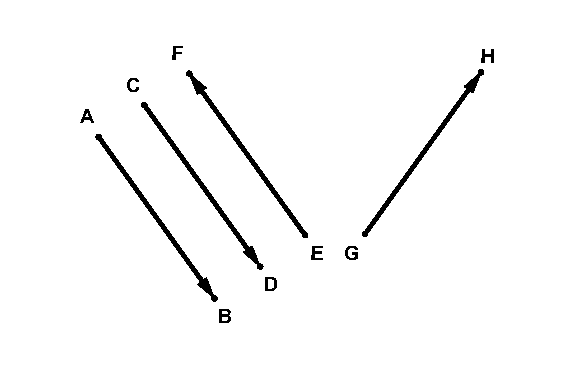
\includegraphics[scale=0.75]{./image/1.1.pdf}
    \caption{}
    \label{fig:1.1}
\end{figure}

与给定箭头相等的所有箭头的集合,称为该箭头的(几何)矢量,通常用符号$\bb{v}$表示。矢量是等价类的一个例子,按照惯例,矢量表示为等价类中任意一个箭头。

等价类,它是一个比你想象的还要更为你所熟知(并且有用)的概念。现在假设我们希望在计算机上对有理数做精确的算术运算。那么比如说,$\frac{2}{3}$就必须以$(2,3)$这样的有序对形式被计算机所读取。我们通过判断是否$ad=bc$,来测试存储在计算机中的两对有序整数$(a,b)$和$(c,d)$的等价性。这样做时,我们默认使用有理数$a/b$的定义作为所有有序整数对$(c,d)$的等价类,使得ad = be。

在实践中,将一个“数字”(如三分之二)与它的各种表示方法(如2/3、4/6等)混用是很方便的(而且很少会引起问题)。同样,当我们使用术语“矢量”时,我们指的是一个“箭头”(反之亦然),这需要读者依靠上下文来做出正确的解释。因此,在图\eqref{fig:1.2}中,我们称任何一个等价的箭头为矢量$\bb{v}$。

\begin{figure}[htbp]
	\centering
	\includegraphics[scale=1.3]{./image/1.2.pdf}
	\caption{}
	\label{fig:1.2}
\end{figure}

矢量的长度$\bb{v}$由$\left| \bb{v} \right|$表示,并定义其为任意一个箭头的长度。零矢量$\bb{0}$是具有零长度的唯一矢量。我们称单位矢量
\begin{equation}
    \widehat{\bb{v}}=\frac{\bb{v}}{\left| \bb{v} \right|},\bb{v}\ne 0
\end{equation}
为矢量$\bb{v}$的方向矢量;零矢量$\bb{0}$没有方向。

我们可以任意在$E_3$中选择一点$O$,并将其称为原点。从点$O$到点$P$(的箭头)的矢量$\bb{x}$称为$P$的位置。我们有时将“位置是$\bb{x}$的点$P$”简写成$P(\bb{x})$。